\chapter{Introduction}

\subsection{Our Contributions}

We propose hyper-lambda-calculi.
Instead of lambda-terms in ordinary lambda-calculi,
we use a finite sequence of lambda-terms called hyper-lambda-terms.
We give three such examples, the first two model asynchronous waitfree
communication and
the other models synchronous send--receive communication.
We also give an example of hyper-lambda-calculi style programming in Haskell.

\citet{hosoi-ono} declared that they chose to study intermediate
logics in
general rather than studying specific intermediate logics.
Concrete results about specific subjects matter when the results
contain new phenomena.
This thesis is intended to contain such a concrete discovery
about specific intermediate and substructural logics.
An intermediate logic is a logic \textit{between} classical and
intuitionistic logics, where `between' is defined using the
set-theoretic inclusion of valid logical formulae of each logic.

Our subject, G\"odel--Dummett logic, is
a typical intermediate logic logic known from 1950's.
Our method is the Curry--Howard correspondence, also known from 1940's.
Our result is characterization of waitfreedom, a concept in the theory
of distributed computation extensively studied in 1990's.
Since both sides of the correspondence is already known,
the discovery is a replay of Curry's surprise.

According to \citet[p.97]{curryhoward},
the Curry--Howard isomorphism~\citep{curryhoward} was first made
precise by \citet[\textbf{9}E and
\textbf{9}F]{curry1974combinatory}.
The intuitionistic propositional logic and the typed lambda calculus
had been independently invented but Curry discovered them to be the same thing.
The ``double discovery'' (\citet{wadler2012propositions}) is considered
to affirm the importance of the typed lambda calculi.
In this thesis we witness a replay of the ``double discovery'' with
different casts: G\"odel--Dummett logic and the waitfreedom.
Both of these were born in the early eras of their respective academic
disciplines:
mathematical logic bore G\"odel Dummett logic in
1950's~\citep{dummett59}
and the computer science bore waitfree computation in
1970's~\citep{lamport1979make}.
This thesis is about the unknown connection between these two.

Of course, there have been many instances of Curry--Howard correspondence.

We list our contributions from the most important: \fix{reorder}
\begin{enumerate}
 \item identifying the computational ability of the
G\"odel--Dummett logic with waitfreedom (Chapter~\ref{ch:lambda});
 \item developing a lambda calculus using
       a hypersequent calculus (Chapter~\ref{ch:lambda});
 \item identifying the communication performed by the prelinearity axiom
       of monoidal t-norm logic (Chapter~\ref{ch:pole});
 \item developing a parametricity argument for
       concurrent processes performing waitfree communication
       (Chapter~\ref{ch:pole}); and
 % \item identifying the communication performed by a seemingly unknown axiom
 %       $(p\limp q)\otimes(q\limp p)$ on top of multiplicative linear
 %       logic (Chapter~\ref{ch:exchange}),
 \item finding a method for implementing hypersequent-based lambda calculi in a
       functional programming language Haskell on the Glasgow Haskell
       Compiler (Chapter~\ref{ch:haskell}).
\end{enumerate}

Our first contribution is finding a way to interpret proofs in
G\"odel--Dummett logic as
concurrently executable programs for waitfree computation.
Although \citet{avron91} noticed his hypersequent calculus has something
to do with concurrency (as the title of~\citep{avron91} contains the phrase
``intermediate logics for concurrency''), it was unknown that
the computational interpretation of G\"odel--Dummett logic has
the degree of synchronization called waitfreedom.  This discovery
constitutes our first contribution.

This is important because it is the first such computational
interpretation for intermediate logics (Fig.~\ref{fig:lattice}).
Another significance of this contribution
is giving interpretation of nondterminism in typed
lambda calculi.  In the simply typed lambda calculus for intuitionistic
propositional logic, all typed terms have a unique normal form.
However, in typed lambda calculi for classical propositional logic,
there can be multiple normal forms unless we employ an evaluation
strategy or limit the set of reductions.
The lack of unique normal forms in the classical propositional proofs
has puzzled logicians for decades. \fix{mention Lafont's example; say it
is a matter of concurrency}
 \begin{figure}
  \centering
  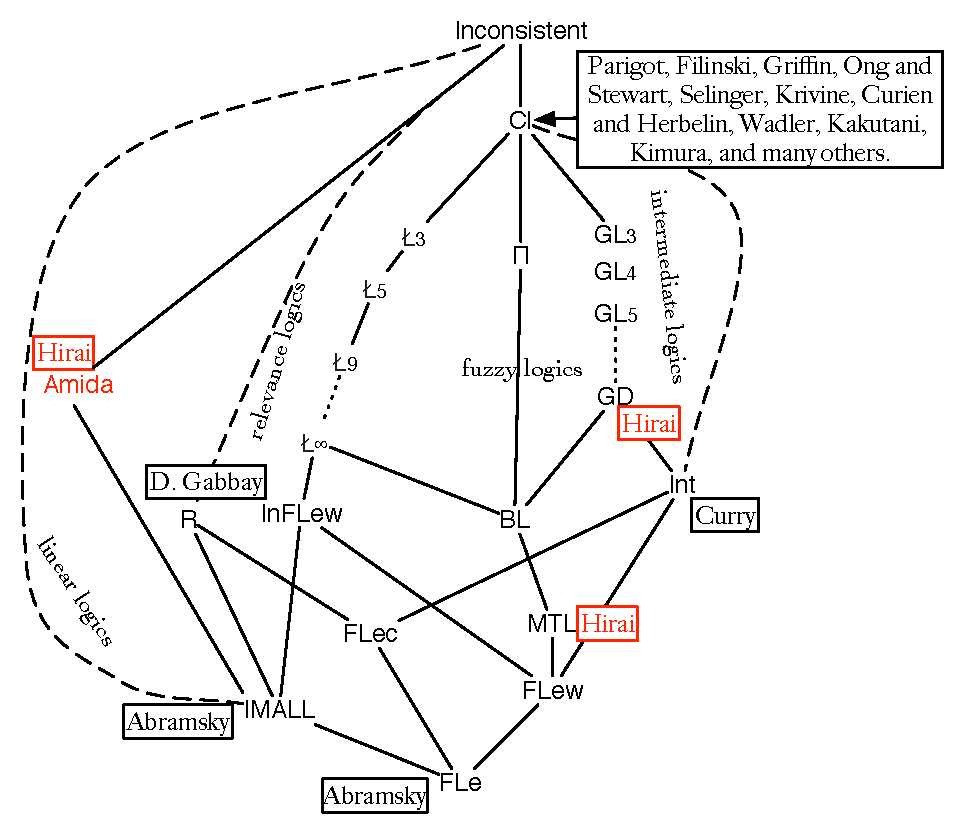
\includegraphics[scale=0.8]{lattice.eps}
  \caption[The substructural logics with lambda calculi.]
  {The substructural logics for which lambda calculi are found.
  The underlying Hasse diagram of well-known substructural logics is
  taken from
  \cite[p.~120]{residuated} with slight modifications.
  The names in boxes refer to people who developed lambda-calculi for
  these logics.
  \textsf{GD} stands for G\"odel--Dummett logic, for which
  a lambda calculus will be given in
  Chapter~\ref{ch:lambda}.
  \textsf{Amida} stands for the Amida logic, an original logic
  defined in Chapter~\ref{ch:exchange}.
  \textsf{MTL} stands for monoidal t-norm logic~\citep{Esteva2001271},
  for which a lambda calculus will be given
  in Chapter~\ref{ch:pole}.
  \textsf{FLe} is for the full Lambek calculus with exchange
  rule~\citep[p.86]{residuated}, which is also known as the
  intuitionistic
  multiplicative additive fragment of linear logic (IMALL).
  \textsf{MALL} stands for its classical version, the multiplicative
  additive fragment of linear logic.  For these fragments of linear
  logic,
  \citet{abramsky1993computational} gave lambda calculi.
  \textsf{R} stands for relevance logic~\citep{urquhart1972},
  for which \citet{gabbay1992} gave a lambda calculus.
  \textsf{Int} stands for the intuitionistic propositional logic.
  The original Curry--Howard isomorphism was found for this logic by
  Curry~\citep{curry1942}.
  \textsf{Cl} stands for the classical propositional logic.
  There is intensive research going on for the computational
  interpretation of classical logic.  Namely,
  Parigot's $\lambda\mu$-calculus~\citep{lambdamu},
  Filinski's symmetric lambda calculus~\citep{filinski1989},
  Griffin's control perator~$\mathcal C$~\citep{griffin1990},
  Ong and Stewart's $\lambda\mu_{\mathrm
  v}$~\citep{ong-stewart},
%   \citet{bb1994}, this is predicate logic
  Selinger's categorical semantics and duality
  result~\citep{selinger2001} for which \citet{kakutani2002} introduced
  fixed-point
  operators,
  Curien and Herbelin's $\bar\lambda\mu\tilde\mu$
  calculus~\citep{curien2000},
  Wadler's dual calculus~\citep{wadler-dual, wadler-reloaded} and so on.
  For the history of lambda calculi for classical logic,
  Daisuke Kimura's thesis~\cite{kimura} is a source of detailed
  information.
  \textsf{Inconsistent} stands for the logic of all logical formulae.
  A programming language \texttt{Haskell}, which is based on
  the typed lambda calculi, has
  an inconsistent type system.
  \fix{add other works mentioned in the picture}
  }
  \label{fig:lattice}
 \end{figure}

Our second contribution is the technique for our first contribution.
We developed a lambda calculus based on \citet{avron91}'s hypersequents.
\citet{avron91} himself noted that it would be important to develop a
lambda calculus for hypersequents.
The lambda calculus relies on \citet{avron91}'s hypersequents.
The hypersequent calculus is a
variant of the deduction system called sequent calculus.  In sequent
calculus, each step of a proof tree concludes a sequent $\G\vdash\phi$ that
consists of a finite sequence of logical formulae~$\G$ and a logical
formula~$\phi$.  The sequent $\G\vdash\phi$ is
interpreted as an implication.  In hypersequent calculus, each step of a
proof tree concludes a hypersequent instead of a sequent.  A
hypersequent is a sequence of sequents delimited by $\hmid$:
$\G\vdash\phi\hmid \D\vdash\psi
\hmid \cdots$.  Also here, each component is interpreted as an
implication, and then the whole hypersequent is interpreted as the
disjunction of all those implications.
When we interpret proofs as programs, we take the components as
concurrent processeses.  Following the original disjunctive
interpretation of components, we regard the proof tree as the guarantee of
success of at least one process.

Our third contribution finds the computational interpretation of
the prelinearity axiom\index{axiom!prelinearity}\index{prelinearity}
$(\phi\limp\psi)\oplus(\psi\limp\phi)$, which is the linear version of
Dummett's axiom.  \fix{add words}

Our fourth contribution is about the parametricity in the second-order
setting.  When we allow logical formulas to have quantifiers on
propositional variables (e.g. $\forall X(X\imp X)$), the logic gets much
more expressive.
Moreover, these second-order types can give more detailed specification
of programs than just specifying the types of outputs given types of
inputs.
For example, in \fix{specify logic}, a term of type $\forall X(X\imp X)$
must be the identity function.
Intuitively, since the term has to work on any type~$X$, the term cannot
``look inside'' \fix{cite something for this phrase} the data of type~$X$.
Using this technique, we find the common behaviour of terms of type
$\forall X \forall Y ((X\limp Y)\oplus (Y\limp X))$, thus finding the
computational semantics of Dummett's axiom.
Our technical development here is very similar to that of
\citet{danos-krivine}.  The crucial difference is that the processes do
not communicate in the case of \citet{danos-krivine} but they perform
waitfree communication in our case.

Our fifth contribution is a confirmation of our first and second
contributions.
We implemented the lambda calculus on top of
Glasgow Haskell Compiler.


\fix{turn this into a table, linear or intuitionistic, conjunction or disjunction}
The previous works treated the computational interpretations of
disjunctive formulae like $(\phi\imp\psi)\lor(\psi\imp\phi)$ or
$(\phi\limp\psi)\oplus(\psi\limp\phi)$.  In this chapter, we try
replacing these disjunctions with conjunctions.
In the former case, the change renders the logic inconsistent.
If we add the axiom $(\phi\imp\psi)\land(\psi\imp\phi)$ to the
intuitionistic propositional logic,
we can prove any formula.  However in the lattar case, the change does
not make the system meaningless.
In this chapter, we treat
the axioms of the form $(\phi\limp\psi)\otimes(\psi\limp\phi)$
on top of IMLL2, the second order formulation of intuitionistic
multiplicative linear
logic.  In essence, the axiom allows two processes to wait for one
another and then exchange information.


The content of Chapter~\ref{ch:lambda} appears in
a conference paper by the author \citep{hiraiflops2012}
although we have applied substantial modifications since then.

% \section{An Introduction for Computer Scientists}

% \section{An Introduction for Proof Theorists}

% \section{An Introduction for Functional Programmers}

% \section{An Introduction for Philosophers}

